\chapter{Desarrollo del Modelo Matemático e Interfaz}
\par En este capítulo se describirá el algoritmo desarrollado para el cálculo de las variables que determinan el proceso de transferencia de calor en cada sección del horno, haciendo referencia a las ecuaciones y los métodos de aproximación antes descritos. También se describirá la interfaz gráfica diseñada para interactuar con el simulador y consistente en pantallas de introducción de datos y pantallas para mostrar los resultados del simulador.

\section{Algoritmo}
\par El diagrama mostrado en la Figura \ref{fig:diagrama-algo}, representa la secuencia del algoritmo. Consta de un ciclo externo que incluye una sección de combustión, sección de radiación, sección de escudo y sección de convección. Su descripción será desarrollada en las subsecciones consiguientes.
\begin{figure}[hbt]
\begin{center}
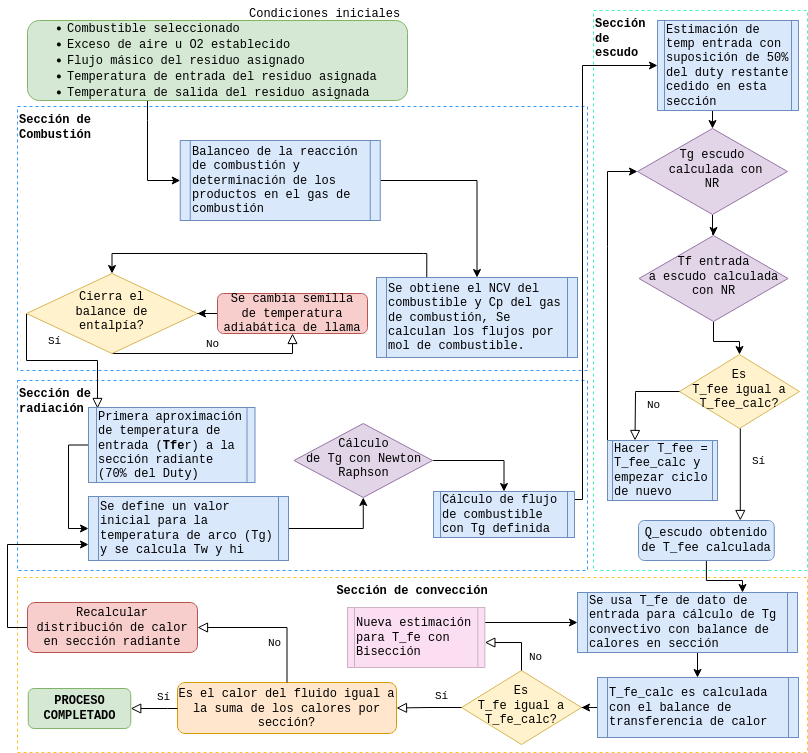
\includegraphics[scale=0.45]{images/diagrama-algo}
\caption[Diagrama de algoritmo]{Diagrama descriptivo del algoritmo desarrollo para el simulador.}
\label{fig:diagrama-algo}
\end{center}
\end{figure}

\par Datos iniciales que recibe el simulador (no todas editables en la interfaz):
\begin{itemize}
    \item Propiedades del fluido, flujo volumétrico, gravedad especifica, calor especifico, conductividad térmica, viscosidad y temperatura, para la entrada y salida.
    \item Composición y temperatura del combustible.
    \item Composición, humedad relativa y temperatura del aire atmosférico.
    \item Configuración y dimensiones del horno.
    \item Propiedades y dimensiones de los tubos y aletas.
\end{itemize}

\subsection{Sección de combustión}
\par En esta sección se ejecutan los cálculos de toda la energía que entra al horno a través de un balance de masa y energía sobre el combustible.
\par Las propiedades del combustible y del gas de combustión resultante, como capacidad calorífica especifica, peso molecular, viscosidad y conductividad térmica, se calculan a partir de las temperaturas, de entrada o por zona, y las fracciones molares de sus componentes individuales.
\par En el simulador se programaron funciones cuadráticas para obtener la viscosidad y conductividad de los componentes del gas de combustión, con dependencia en la temperatura, en caso de la capacidad calorífica se usa la ecuación cúbica mostrada en el libro de Borgnakke y Sonntag\cite{bib:vanwylen}, los coeficientes para cada una de las propiedades se calcularon con los datos del Instituto Nacional de Estándares y Tecnología (NIST)\cite{nist}, el código desarrollado para las ecuaciones se encuentra en los apéndices. 
\par Finalmente se calcula la relación aire/combustible con la ecuación \ref{eq:ac}, la temperatura adiabática de llama y el poder calorífico neto del combustible (NCV) de la ecuación \ref{eq:pc}.


\subsection{Cálculo térmico del horno}
\par Aquí se utiliza un ciclo encargado de recibir todos los parámetros de entrada y correr cada una de las subsecciones como funciones, es donde se define la distribución de calor entre las secciones del horno y varia este valor para alcanzar la tolerancia deseada con un método iterativo aplicado a la siguiente ecuación.
\begin{equation}
\label{eq:ciclo_externo}
\frac{(Q_{residuo} - Q_{calc})}{Q_{calc}} \approx 0
\end{equation}
\par Donde:\\
$Q_{residuo} = m_{residuo} * C_{p_residuo} * {\Delta}T_{residuo}$ \\
$Q_{calc} = Q_{RAD} + Q_{ESC} + Q_{CONV}$ \\
$Q$ = Calor transferido. \\

\par Lo que se traduce en que el calor absorbido por el residuo debe ser igual al calor suministrado en cada una de las secciones del horno.
\par El valor inicial de distribución radiante esta definido en 64\% y esta converge para el rango de temperaturas permitido en la interfaz del simulador. En las siguientes subsecciones se detallan las ecuaciones para cada etapa del horno.

\subsection{Sección de radiación}
\par Tres variables quedan por determinar en esta sección $Q_{RAD}$, la temperatura de entrada del fluido a la zona $T_{fer}$ radiante y la temperatura efectiva del gas $T_g$.

\par \textbf{Suposición A}: Para obtener un primer valor de la temperatura de entrada del residuo de vacío a esta sección se supone una absorción del calor del horno ($Q_{absorbido}$) como 70\% en la zona radiante y el 30\% entre la zona escudo y zona convectiva, en consecuencia (ec. \ref{eq:sup-a}):
\begin{equation}\label{eq:sup-a} Q_{RAD} = 0.7 * Q_{absorbido} \end{equation}
\par El $Q_{RAD}$ supuesto corresponde al valor inicial de un procedimiento de ensayo y error que cierra con al obtener un $Q_{absorbido}$ calculado ($Q_{RAD} + Q_{ESC} + Q_{CONV}$) igual al $Q_{absorbido}$ especificado. A partir de $Q_{RAD}$ se pueden estimar las siguientes variables:
\begin{itemize}
\item De la ecuación (\ref{eq:rad-fluid}) se obtiene la temperatura de entrada del fluido a la zona radiante $T_{fer}$ y la temperatura de mezcla $T_b$.
\item Conocida el área de los tubos se obtiene $Flux_R = Q_{RAD} /At$.
\item De la ecuación (\ref{eq:hi}) se obtiene el coeficiente de película $h_i$. Los números de Re y Pr se calculan a $T_b$.
\item De la ecuación (\ref{eq:tw}) se obtiene la temperatura de pared del tubo $T_w$.
\item Con $T_w$ calculada se recalcula $h_i$, incluyendo la corrección por viscosidad y $T_w$.
\end{itemize}
\par Todos los valores calculados dependen del supuesto A, el  posterior ajuste de QR modifica estos valores.
\par Finalmente mediante la ecuación (\ref{eq:rad-tgr}) y usando el Método de Newton Raphson se calcula la Temperatura Efectiva del gas, $T_g$ y mediante la ecuación (\ref{eq:rad-comp}) el consumo  de combustible correspondiente a la suposición A.

\subsection{Sección de escudo}
\par De la zona escudo se conocen tres variables, la temperatura de salida del fluido $T_{fer}$, la temperatura de entrada del gas de combustión $T_{gr}$ = $T_g$ y la cantidad de calor por radiación que escapa hacia la zona escudo $Q_{radEsc}$. Son incógnitas la temperatura de salida del gas $T_{ge}$, la temperatura de entrada del fluido $T_{fee}$ y el calor transferido $Q_{ESC}$.
\par \textbf{Suposición B}: Suponer la temperatura de entrada del fluido de la zona escudo $T_{fee}$. Recurriendo nuevamente al calor absorbido especificado, el 30\% se transfiere en la zona escudo y la zona convectiva por la suposición A, si consideramos que en el escudo se absorbe el calor por radiación que escapa de la zona radiante lo que en cierta forma compensa la menor área de transferencia en comparación con la zona convectiva, como una razonable aproximación (ec. \ref{eq:sup-b}) se supone que:
\begin{equation} \label{eq:sup-b} \begin{gathered}
    Q_{ESC} \approx Q_{CONV} \approx 0.15 * Q_{absorbido}\\
    Q_{ESC_{sup}} = 0.15 * Q_{absorbido} 
\end{gathered} \end{equation}
\par Esto conlleva a un valor inicial para el ensayo-error de $T_{fee}$ = ($T_{fer}$ +$T_{fe}$)/2. 

\begin{itemize}
\item A partir de la ecuación (\ref{eq:esc}) calcular la temperatura de salida del gas $T_{ge}$.
\item Calcular la temperatura de mezcla del gas $T_{gb}$ y del fluido $T_{fb}$.
\item Calcular LMTD mediante la ecuación (\ref{eq:qesc-lmtd}).
\item Calcular ho, hr, hi mediante las ecuaciones (\ref{eq:hi}), (\ref{eq:ho}) y (\ref{eq:hr}).
\item Calcular Uo.
\item Calcular $Q_{ESC}$ a partir de la ecuación (\ref{eq:tesc}).
\item Calcular $T_{fee}$ a partir de la ecuación (\ref{eq:lmtd}).
\item Comparar $T_{fee}$ calculada con $T_{fee}$ supuesta.
\end{itemize}
\par Si $|\frac{T_{fee_c} - T_{fee_s}}{T_{fee_s}}| > error$, se hace $T_{fee_s} = T_{fee_c}$ y $Q_{ESC_{sup}} = Q_{ESC_{calc}}$ y se regresa al primer punto.
\par Si $|\frac{T_{fee_c} - T_{fee_s}}{T_{fee_s}} | < error$, se da por cerrado el cálculo de la zona de escudo. Al final del proceso $\frac{Q_{ESCcalc} - Q_{ESCsup}}{ Q_{ESCsup}}$ debe estar en un valor cercano a cero.

\subsection{Sección de convección}
\par En la zona conectiva las variables conocidas provenientes del cálculo de la zona Radiante y Escudo son la temperatura del gas a la entrada $T_{ge}$ y la temperatura de salida del fluido $T_{fee}$.
\par \textbf{Suposición C}: Para tener solo una temperatura como incógnita en el cálculo se supone la temperatura de entrada del residuo de vacío al horno, $T_{fe}$, igual al valor especificado en el ingreso de datos y se procede a:
\begin{itemize}
\item Calcular la temperatura de salida del gas $T_{gc}$ y el calor transferido $Q_{CONV}$ correspondiente mediante la ecuación (\ref{eq:conv}).
\item Calcular temperatura de mezcla del gas y del fluido.
\item Calcular LMTD.
\item Calcular Uo, según las ecuaciones descritas para tubos con aleta.
\item Calcular $Q_{CONV_{calc}}$ a partir de la ecuación (\ref{eq:qconv}).
\end{itemize}
\par Si $|\frac{Q_{CONVcalc} - Q_{CONVsup}}{Q_{CONVsup}} | > error$ se recalcular la temperatura de entrada del fluido $T_{fe}$ usando el método de bisección y se vuelve al punto inicial de la sección.
\par Si $|\frac{Q_{CONVcalc} - Q_{CONVsup}}{Q_{CONVsup}} | < error$, se cierra el cálculo en la zona convectiva.
\par Las variables calculadas al finalizar el procedimiento son  $Q_{CONV}$, $T_{fe}$ y $T_{ge}$.

\subsection{Cierre del algoritmo de cálculo del horno}
\par A este nivel de avance se han calculado $Q_{RAD}, Q_{ESC}, Q_{CONV}$ y todas las temperaturas excepto la temperatura del fluido a la salida del horno $T_{fs}$, la cual se ha mantenido igual a la especificada. El control del proceso de simulación vuelve al ciclo externo y dos comprobaciones con los valores calculados son posibles:\\
\par ¿Es la temperatura de entrada $T_{fe}$ calculada $>, <$ ó = a la $T_{fe}$ especificada?
\par ¿Es $Q_{RAD} + Q_{ESC} + Q_{CONV} >, <$ ó = al $Q_{absorbido}$?\\
\par Ambas están relacionadas y se abre el siguiente flujo condicional para manejar los tres escenarios:
\begin{itemize}
    \item Si $|\frac{T_{fe_{calc}} - T_{fe_{sup}}}{T_{fe_{sup}}} | > error$ y si $T_{fe_{calc}} > T_{fe_{sup}}$ entonces $Q_{RAD} + Q_{ESC} + Q_{CONV} < Q_{absorbido}$. Aumentar el calor transferido en la zona radiante y repetir todo el proceso de cálculo desde la sección de radiación. El resultado será el incremento de la temperatura efectiva $T_{g}$ y su efecto aguas abajo en la zona escudo y convectiva.
    \item Si $|\frac{T_{fe_{calc}} - T_{fe_{sup}})}{T_{fe_{sup}}} | > error$ y si $T_{fe_{calc}} < T_{fe_{sup}}$ entonces $Q_{RAD} + Q_{ESC} + Q_{CONV} > Q_{absorbido}$. Disminuir la distribución del calor transferido a la zona radiante y volver a la sección radiante para repetir los cálculos con esta nueva suposición. El resultado será que decrece la temperatura efectiva $T_{g}$ y su efecto aguas abajo en la zona escudo y convectiva.
    \item Si $|\frac{T_{fe_{calc}} - T_{fe_{sup}})}{T_{fe_{sup}}} | < error$ entonces también $|Q_{RAD} + Q_{ESC} + Q_{CONV} - Q_{absorbido}|$ es menor al error establecido, se considera correcta la suposición A.
\end{itemize}
\par Se continua a reportar los resultados y finaliza el algoritmo.

\section{Interfaz de usuario}
\par Una interfaz de usuario (UI de su término comúnmente usado inglés) es el medio por el cual una persona controla una aplicación de software o dispositivo de hardware. Esto significa que el programa incluye controles gráficos que optimizan la experiencia de usuario usando un ratón, teclado o pantalla táctil.
\par Los elementos más comunes de una interfaz gráfica de usuario, de acuerdo con Career Foundry\cite{ui}, son:
\begin{itemize}
\item Controles de entrada: permiten introducir información en el sistema por parte de los usuarios.
\item Componentes de navegación: ayudan a los usuarios a moverse.
\item Componentes informativos: brindan información a los usuarios.
\item Contenedores: mantienen el contenido organizado, como paneles, ventanas, marcos, etc.
\end{itemize}

\par La interfaz de usuario implementada para el algoritmo se desarrolló usando los lenguajes básicos de desarrollo web, Lenguaje de Marcado de Hipertexto (HTML), Hojas de Estilo en Cascada (CSS) y el lenguaje de programación interpretado JavaScript (JS), lo que hace que sea totalmente editable y pueda correr en cualquier ordenador o dispositivo móvil con navegador web sin instalar otro programa.

\subsection{Descripción de uso y alcances}
\par Esta vista otorga instrucciones y limitaciones de uso del simulador, al ser la vista principal el usuario podrá conocer todas las capacidades y aplicaciones disponibles en la versión actual publicada (ver la Figura \ref{fig:alcance}).
\par Aquí se describen las condiciones de operación simulado para dar una referencia al usuario de las cargas que puede manejar el simulador dentro de los rangos reales de uso.

\subsubsection{Condiciones de Operación}
\begin{itemize}
\item \textbf{Diseño}: 23.0 MW (78.79 MMBtu/h) - Máxima capacidad de procesamiento.
\item \textbf{Normal}: 20.9 MW (71.5 MMBtu/h) [90,75\% del Diseño] - Operación habitual del horno.
\item \textbf{Turndown}*: 10.45 MW (35.77 MBtu/h) [45,4\% del Diseño] - Condición de mínima capacidad.
\end{itemize}

\par *No equivale a una condición de "turndown" de los quemadores puesto que podría lograrse con cierto número de quemadores operando normalmente y otros quemadores simplemente apagados.

\subsection{Introducción de datos}

\par En esta sección se desarrollan dos vistas, (Fig. \ref{fig:datos} y Fig. \ref{fig:fulldatos}) una simplificada para introducir solo los datos más relevantes del proceso y que dirige a una pantalla de resultados donde se pueden comparar dos estados; otra donde se observan todas las variables que permite modificar el proceso y esta a su vez tiene dos opciones de resultados, una pantalla de valores numéricos detallados y una segunda pantalla que muestra una variación gráfica en el rango de cuatro variables a escoger.  

\subsection{Resultados ampliados}

\par En esta vista se detallan todas las variables resultantes por cada sección del horno (Fig. \ref{fig:fullresultados}), se puede escoger el sistema de unidades a expresarse en la pantalla anterior.
\par El objetivo de esta vista es tener una visión del comportamiento de todas las variables en el proceso, de aquí se pueden encontrar explicaciones no tan obvias del comportamiento de las variables finales mostradas en la vista comparativa.

\subsection{Resultados comparativos}

\par Esta es la vista que aspira ser más educativa al resumir todas las variables resultantes y hacer una comparación entre dos condiciones de operación (Fig. \ref{fig:resultados}).
\par Aquí se puede observar rápidamente los cambios en variables particulares y de interés, como los datos de ingreso, las emisiones de \ac{co2}, el consumo de combustible, la distribución de calor dentro del horno, la temperatura de salida de los gases de combustión y la eficiencia térmica.

\subsection{Gráficas de tendencias}

\par El propósito inicial de esta sección fue generar una visual del comportamiento del horno simulado a lo largo de un rango, se uso para conseguir zonas donde los métodos aproximados del simulador no convergían y permitió sintonizar el paso, numero de iteraciones, valor inicial y tolerancia de dichos métodos.
\par Luego de ser optimizada ahora permite observar la tendencia de las variables de salida seleccionadas con precisión, facilitando la comprensión de los resultados de los fenómenos dentro del horno (Fig. \ref{fig:graficas}).